When CMake projects get big, configuring them might take quite a long time, especially if there is external content loaded or if there are lots of checks done for toolchain features. A first step to optimize this is to check what part of the configuration process takes up how much time. Since version 3.18, CMake includes command-line options to produce nice profiling graphs to investigate where the time is spent during configuration. By adding the -{}-profiling-output and --profiling-format profiling flags, CMake will create profiling output. At the time of writing this book, only the Google trace format for the output format is supported. Despite this, the format and the file need to be specified to create the profiling information. A call to CMake to create a profiling graph could look like this:

\begin{tcblisting}{commandshell={}}
cmake -S <sourceDir> -B <buildDir> --profiling-output
./profiling.json --profiling-format=google-trace
\end{tcblisting}

This will write the profiling output to the profiling.json file in the current directory. The output file can be viewed with Google Chrome by typing about://tracing into the address bar. A tracing output for a cached build of the GitHub project to this book could look like this:

\begin{center}
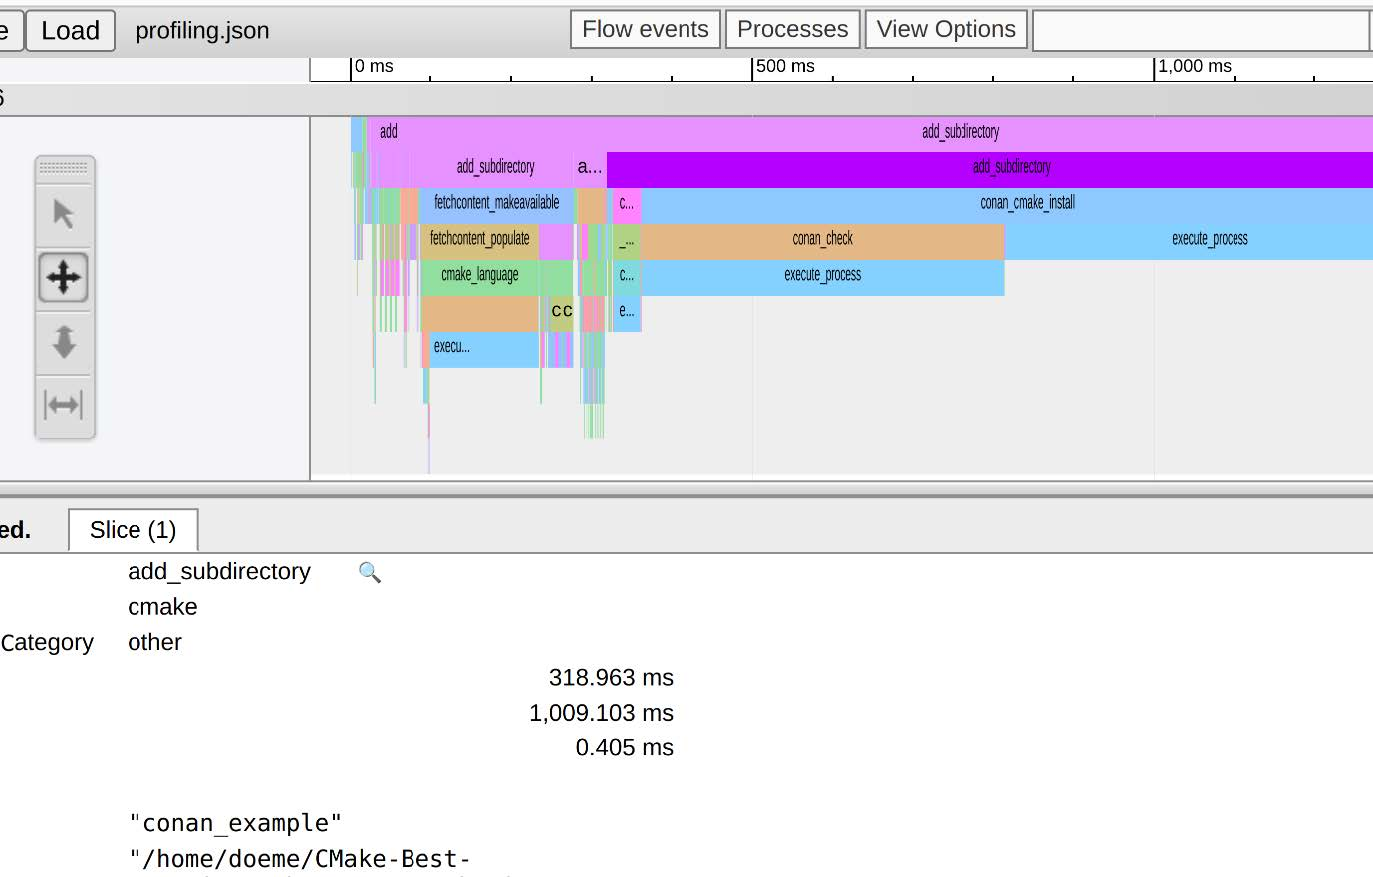
\includegraphics[width=0.8\textwidth]{content/3/chapter14/images/1.jpg}\\
Figure 14.1 – An example profiling graph for a CMake project displayed in Google Chrome
\end{center}

In the preceding figure, it is pretty obvious that there is one call to add\_subdirectory that takes up the majority of the time when configuring the project. In this case, this is the chapter\_5 subdirectory, taking a bit more than 3 seconds to complete. By drilling down a bit, it becomes apparent that these are the examples that use the Conan package manager, namely the two calls to conan\_cmake\_install that make the configuration relatively expensive. In this case, centralizing the calls to Conan in a directory further up would cut the time CMake would take for a configuration run in half.

In order to correctly interpret the profiling output, it helps to compare different runs of CMake with each other, especially comparing CMake running on a clean cache with one that makes use of cached information. If only the CMake runs on a clean cache take their time, but the incremental runs are fast enough, this might still be acceptable for the developers. However, if the incremental CMake runs take their time as well, this might be more problematic. Profiling them may help you find out if there are unnecessary steps done for each configuration run.

Fixing slow build steps will depend on the concrete situation, but a common culprit for long configuration times is files that are downloaded each time because there is no check whether the file exists in the first place. Analyzing the profiling calls might often show calls such as execute\_process or try\_compile consuming lots of execution time. The most obvious "fix" would be to try to get rid of these calls, but often these calls are there for a reason. More often, following up the call stack leading to the commands might reveal opportunities to reduce how often these functions will be called. Maybe the results can be cached, or maybe files created with execute\_process do not need to be generated each time.

Especially when cross-compiling, find\_ commands might also take up a lot of time. Changing the search order by changing the various CMAKE\_FIND\_ROOT\_PATH\_MODE\_variables, as described in Chapter 5, Integrating Third-Party Libraries and Dependency Management, might help a bit here. For a more thorough analysis of why the find\_ calls take up too much time, CMake can be told to enable debug output for them by setting the CMAKE\_FIND\_DEBUG\_MODE variable to true. As this will print out a lot of information, it is a good idea to enable this only for certain calls, as follows:

\begin{lstlisting}[style=styleCMake]
set(CMAKE_FIND_DEBUG_MODE TRUE)
find_package(...)
set(CMAKE_FIND_DEBUG_MODE FALSE)
\end{lstlisting}

The profiling options of CMake allow profiling the configuration stage of the build process; profiling the actual compilation and time have to be done by using the respective generator. Most generators either support some profiling option or log the needed information. For Visual Studio generators, the vcperf tool(\url{https://github.com/microsoft/vcperf}) will give a lot of insights. When using Ninja, the .ninja\_log file can be converted into Google trace format using the ninjatracing tool(\url{https://github.com/nico/ninjatracing}). While CMake does not offer support to profile the actual compiling and linking of software, it does offer ways to improve build times, which we will see in the next section.































